% Seção: LLVM

\section{LLVM - Low Level Virtual Machine}
\label{revisao:llvm}

\subsection{Hist\oh ria e motiva\ca o}

Segundo \cite{LLVMorg}, o LLVM\sigla{LLVM}{Do ingl\^es \emph{Low Level Virtual Machine}} come\cc ou como um projeto de pesquisa na universidade de Illinois, nos Estados Unidos, com a meta de fornecer uma estrat\eh gia de compila\ca o moderna, baseada em SSA\footnote{Explicado na se\ca o \ref{revisao:estrutura-geral:geracao-codigo}}, capaz de suportar compila\ca o est\ah tica e din\^amica de linguagens de programa\ca o arbitr\ah rias.

\cite{Machado07} diz que \cite{Lattner02} prop\^os em sua tese o LLVM como uma ferramenta para endere\cc ar o problema de gera\ca o do melhor c\oh digo poss\ih vel\footnote{O problema de gerar c\oh digo \oh timo \eh\ NP-completo \cite{Aho08}.}, levando em considera\ca o a evolu\ca o constante das linguagens de programa\ca o, para assim atingir tr\^es metas:

\begin{enumerate}
\item Permitir otimiza\ca o agressiva em m\uh ltiplos passos;
\item Servir de \emph{host} (como hospedeiro ou infraestrutura) para pesquisa de compiladores e otimiza\ca o; e
\item Operar de forma transparente para o usu\ah rio como um substituto direto a ferramentas como o GCC\sigla{GCC}{\emph{GNU Compiler Collection}}\footnote{\emph{GNU Compiler Collection}, fam\ih lia de compiladores para linguagens C, C++, Objective-C, Java e Fortran.}.
\end{enumerate}

Segundo \cite{Cantu08:1}, o LLVM tem como objetivo executar an\ah lises e transforma\co es\footnote{No sentido de otimiza\ca o de desempenho} ao longo do tempo de vida do programa de forma trasparente para o programador. Neste sentido, podemos entender que se refere a estrat\eh gia de otimiza\ca o em m\uh tiplos passos tomada pela arquitetura do LLVM.

\subsection{Trabalhos derivados}

Diversos trabalhos foram originados do projeto LLVM para diversos objetivos como localiza\ca o de causas-raiz de falha de software\cite{Sahoo13}, aplica\ca o de atualiza\co es de seguran\cc a durante seu funcionamento, reduzindo o \emph{downtime}\cite{Giuffrida13}, detec\ca o de falhas em programas \emph{multi-thread}\cite{Lucia13}, al\eh m de novas linguagens de programa\ca o, por exemplo.

Desde seu in\ih cio, diversas empresas do setor privado tamb\eh m passaram a utilizar as ferramentas do projeto, como Adobe, Apple\footnote{Todas as ferramentas de desenvolvimento das plataformas Apple, incluindo Xcode, MacOSX e iOS utilizam o LLVM para gera\ca o de programas otimizados.}, Intel, NVIDIA, entre outras, segundo \cite{LLVMorg}.

\subsection{Arquitetura do LLVM}

Na figura \ref{fig:llvmarch} podemos ver a arquitetura de construção do projeto LLVM, consitu\ih da pelo \emph{frontend} (um por linguagem de programa\ca o), respons\ah vel pelo processamento e valida\ca o do programa fonte que gera o c\oh digo intermedi\ah rio no formato LLVM-IR\sigla{LLVM-IR}{Do ingl\^es \emph{Low Level Virtual Machine Intermediate Representation}}\footnote{Low Level Virtual Machine - Intermediate Representation\sigla{LLVM}{Low Level Virtual Machine - Intermediate Representation}.}, o \emph{bitcode}\footnote{Originalmente a representa\ca o intermedi\ah ria do LLVM chamava-se \emph{bytecode}, por\eh m, com a evolu\ca o do projeto, prestando suporte a um maior n\uh mero de plataformas e arquiteturas, essa especifica\ca o tornou-se bin\ah ria, mais compacta, tendo seu nome modificado.}, seguido pelos passos de otimização e finalmente o \emph{backend} (um por arquitetura de hardware) que transforma a representação intermedi\ah ria otimizada em c\oh digo objeto, segundo \cite{Dobbs12}.

\begin{figure}[htp]
  \begin{center}
    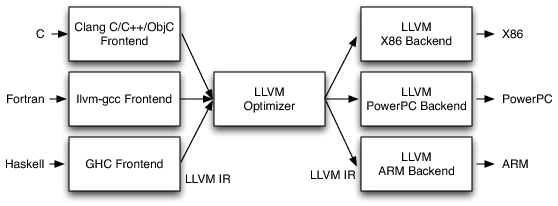
\includegraphics[width=0.7\textwidth]{figuras/llvmarch}
  \end{center}
  \caption{Arquitetura do projeto LLVM}
  \label{fig:llvmarch}
\end{figure}

Na figura \ref{fig:llvmarch2}, vemos mais detalhes de como a arquitetura flex\ih vel do LLVM interage com outros programas e arquivos, realizando a liga\ca o-edi\ca o, otimiza\ca o e otimiza\ca o em tempo de execu\ca o, retirado de \cite{Machado07}.

\begin{figure}[htp]
  \begin{center}
    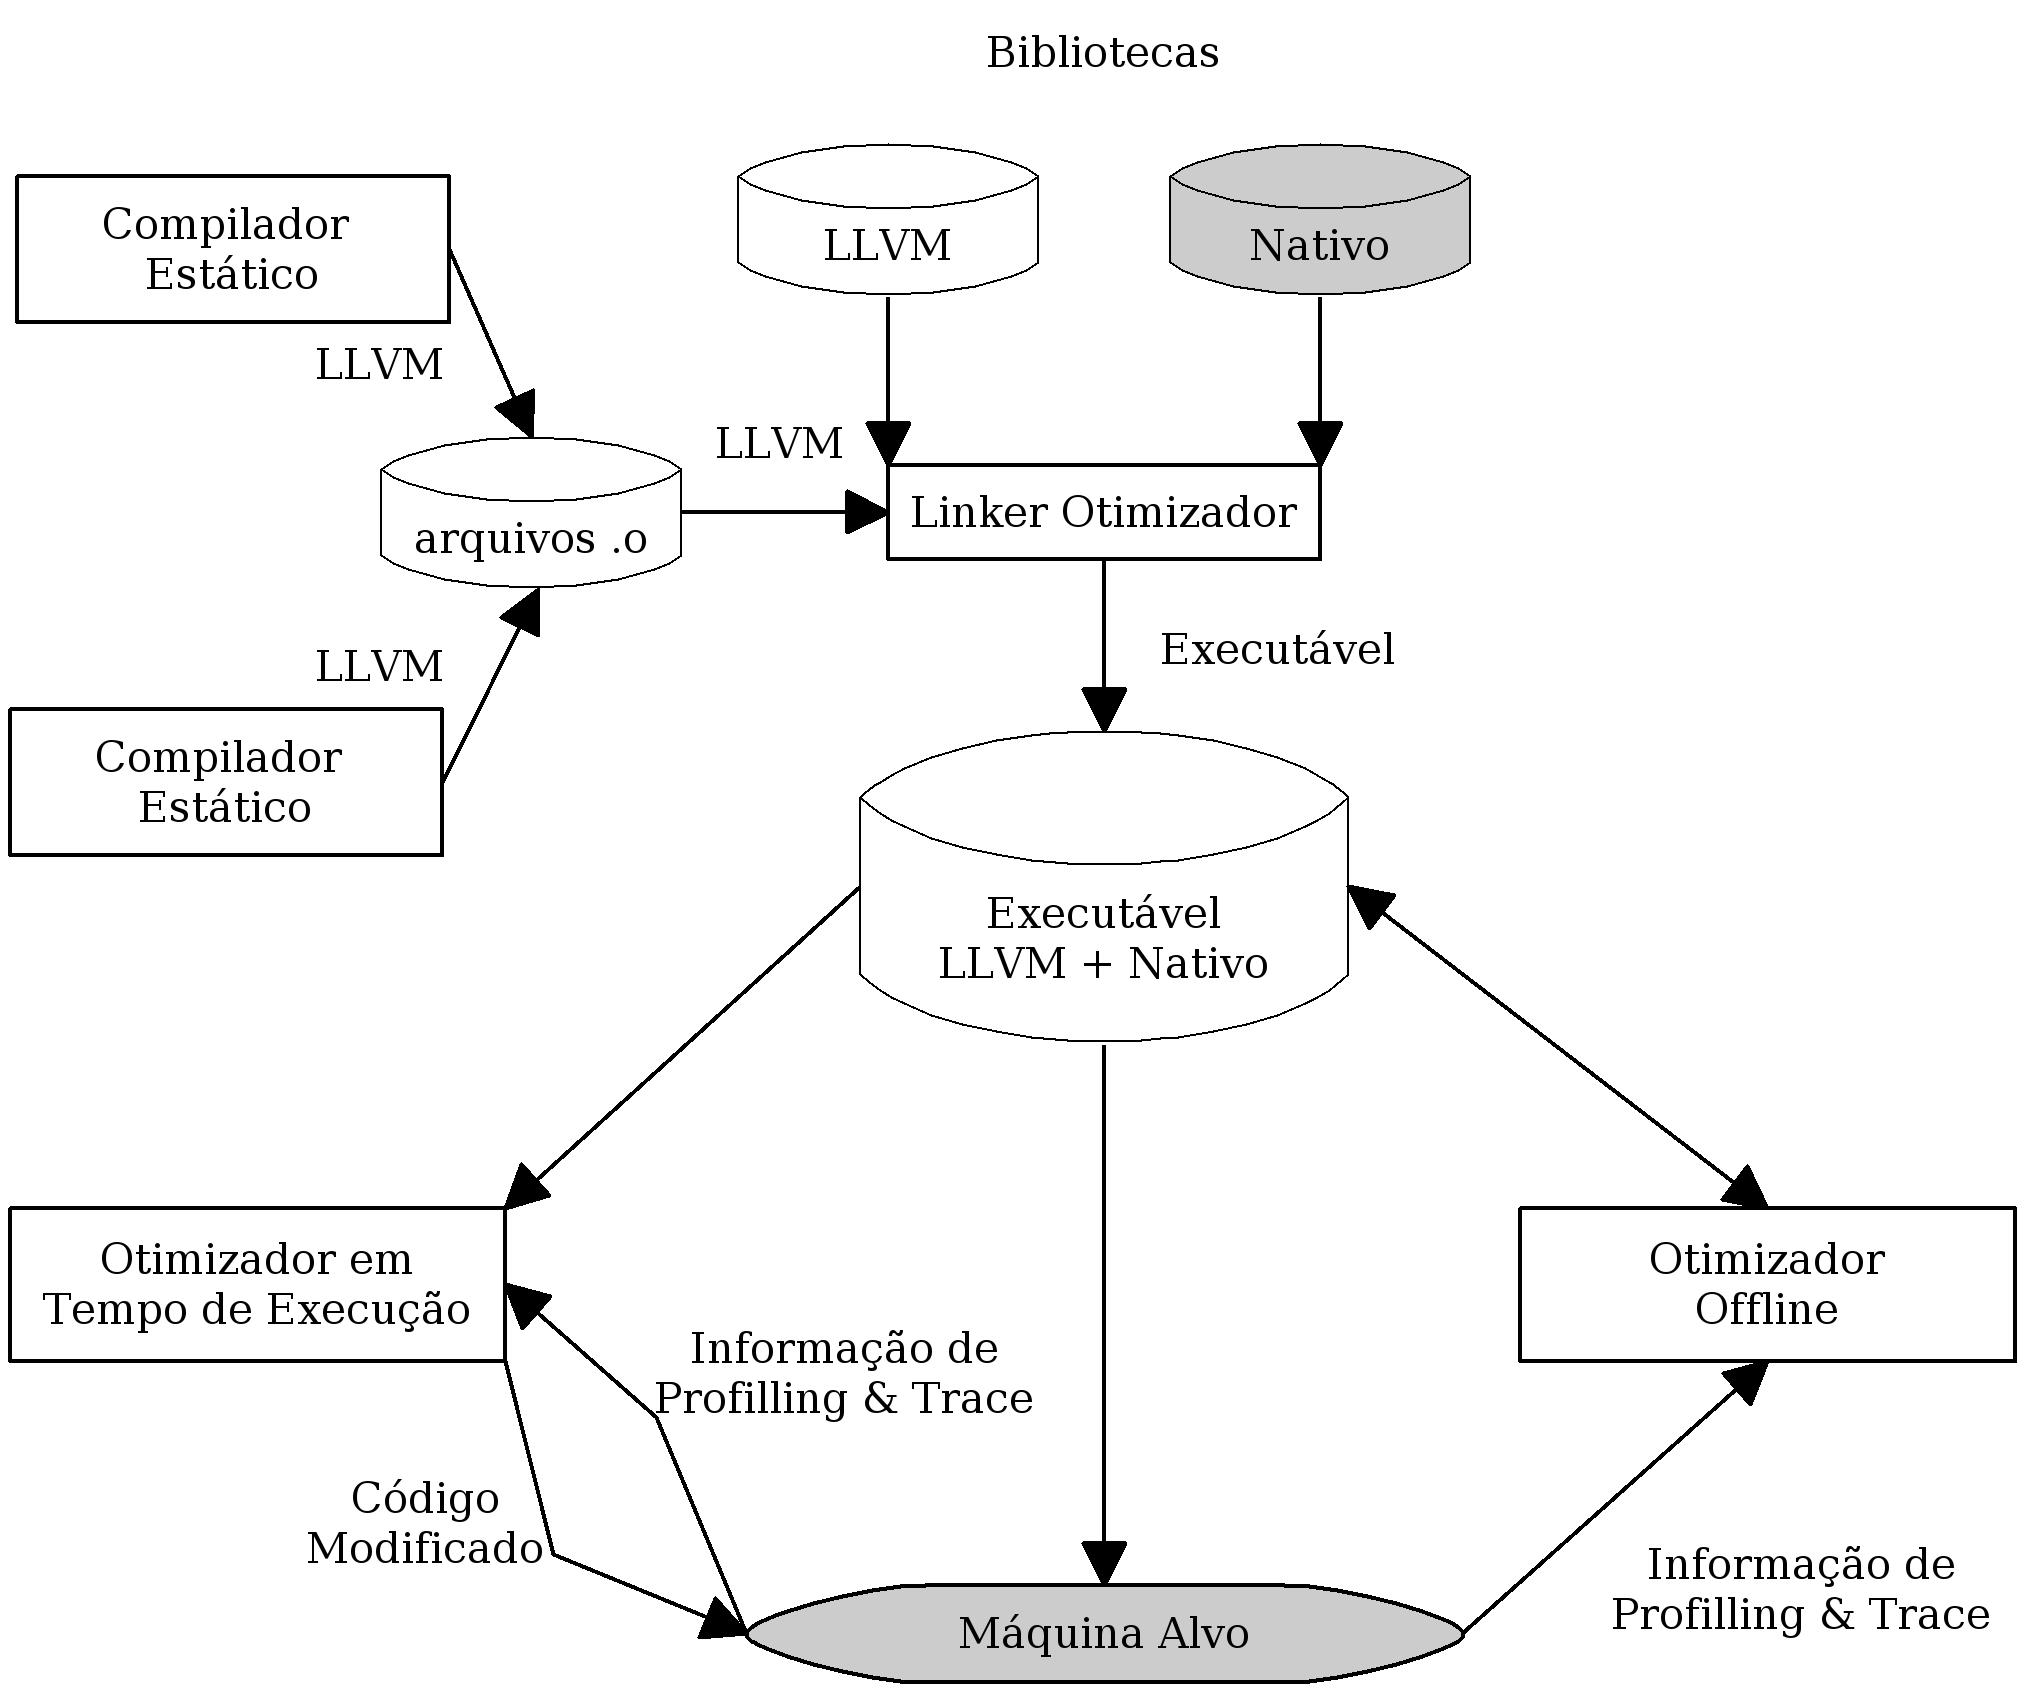
\includegraphics[width=0.7\textwidth]{figuras/llvmarch2}
  \end{center}
  \caption{Arquitetura detalhada do projeto LLVM}
  \label{fig:llvmarch2}
\end{figure}

Aqui podemos notar a estrutura de longa vida que o projeto fornece, permitindo otimiza\ca o de programas mesmo durante sua utiliza\ca o.

\subsection{LLVM-IR - A representa\ca o intermedi\ah ria do LLVM}
\label{llvm:llvm-ir}

Segundo \cite{Cantu08:1}, a representa\ca o intermedi\ah ria do LLVM foi desenvolvida para prover informa\co es de alto n\ih vel suficientes para an\ah lises e transforma\co es, e de baixo n\ih vel suficiente para programas arbritr\ah rios, independentes de plataforma, sendo assim, port\ah teis. Composto por apenas 31 instru\co es, fornece uma representa\ca o fortemente tipada e objetiva para representa\ca o e manipula\ca o de vari\ah veis de tipos primitivos e derivados, ponteiros e fun\co es.

\cite{Machado07} complementa, explicando que a representa\ca o pode ser consumida de tr\^es formas:

\begin{enumerate}
\item Uma em texto leg\ih vel, para inspe\ca o do c\oh digo gerado;
\item Uma interna, em mem\oh ria, acessada via API espec\ih fica; e
\item Uma compactada, chamada de \emph{bitcode}.
\end{enumerate}

% \subsection{Otimiza\ca o em m\'ultiplos passos}
